\subsection{Opgave 14}

En retvinklet trekant er skitseret på figuren.\\\\
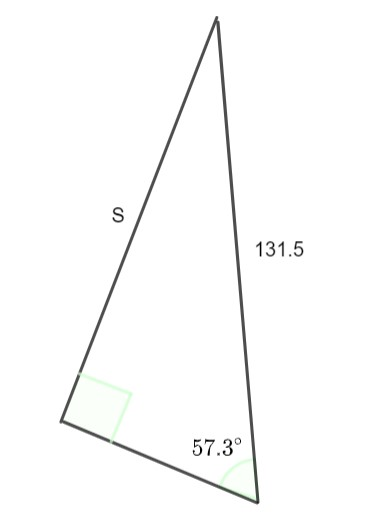
\includegraphics[width=7cm]{Opgave_11-20/Opgave_14/Opgave_14.jpg}\\\\
Bestem længden S.\\\\

\ans
For retvinklede trekanter gælder formlen
\begin{align*}
    \sin(B) = \frac{c}{b}
\end{align*}
Her er B vinklen $B = 57.3^{\circ}$, c er længden af hypotinusen dvd $c = 131.5$ og b er siden som i vores tilfælde svarer til s. Vi isolerer altså b og indsætter tallene
\begin{align*}
    \sin(B) = \frac{b}{c} \Longleftrightarrow b = \sin(B)\cdot c = \sin(57.3^{\circ})\cdot 131.5 \approx 89.76
\end{align*}
